\chapter{基于知识库图嵌入的视觉问答模型}
\section{知识库概述}
人类智能体通过学习和实践不断获取知识与经验,并能将习得的知识存储在记忆系统中,面对相关问题时能准确、快速地调用相关的知识和经验,完成识别和推理过程,成功解决问题。人工智能系统的终极目标便是能像人类一般快速、准确地解决未知问题,甚至超越人类的物理极限,实现范围更广、更艰深的任务解决。人类在真实世界中的学习是不断将非结构化的信息重构为结构化的知识的过程,知识库(KB)是一种包含常识和描述真实世界的事实的知识集,在不同的应用情景中有不同的内部结构。

知识库最早被应用于人工智能中的专家系统\citing{akerkar2010knowledge}。专家系统是一种建立在知识库基础上,使用推理方法完成复杂推理过程,最终实现与人类专家同水平的决策能力的计算机系统,被广泛应用于医学诊断、分子结构推理、自然语言理解等领域。专家系统面向的专家任务需要特定领域的知识,这也使得知识库成为专家系统的核心之一。针对不同领域的任务构建知识的表达方式是困难的,因为专家知识可能是不精确的,同时要从知识库中获取答案的过程依赖于人工的制定复杂的规则,知识库精度和人力成本等因素制约了专家系统在更多领域的应用。

知识库也被应用于在自然语言处理的任务,例如机器翻译和文本问答。知识库中的本体包含某个领域中的各种概念和概念间的关系,本体在机器翻译中可作为知识源\citing{nirenburg1994machine}。语言学中的多义词在不同的语境中被解释为不同的含义,人类能根据上下文语境的不同选择出最恰当的词语,但对于机器翻译系统便是一大难题。当机器翻译系统能够获得足够多的本体作为知识源时,能较好地解决多义词的解释问题,从而得到更加准确的翻译结果\citing{knight1993building}。

文本问答系统在早期作为专家系统的交互界面,在之后的发展中逐渐独立出来成为自然语言处理的一个分支。文本问答系统根据给出的文本问题,从文本知识库中提取答案,此时的文本知识库往往是文本组成的文档,还未使用资源描述框架(RDF)的结构化数据。大多数文本问答系统都采用相对标准的结构:根据问题文本建立查询、利用信息提取方法(IR)确定可能包含答案的文章位置、进一步确定答案所在的片段,这种架构下不使用任何与答案相关的额外知识\citing{hermjakob2000knowledge}。

应用信息提取技术(IR)的问答系统有一个非常明显的缺点——只能根据问题确定答案相关的文章或者段落,不能给出更为直接的答案。为解决这种缺陷,研究人员探索了更多的方法。

Burke等人一改通常的从文章中提取答案的方式,先将被频繁问到的问题(FAQ)以“问题-答案”对的形式存储为知识库,再从新问题中寻找与知识库匹配程度最高的“问题-答案”对,进而获得答案\citing{burke1997question}。在此方法中最核心的步骤是对新旧问题之间的匹配,为了使匹配的问题之间的语义相似度最大,系统还使用了WordNet\citing{miller1995wordnet}的语义知识,WordNet能提供词语和其同义词集合、同义词集合之间的关系,因此能避免一些匹配过程中的歧义错误,提高匹配的准确度。这里以“匹配”为核心思想的算法最大的障碍是常见问题集的容量、深度和广度问题,因此通常对于范围较小的场景而言,才能实现较好的匹配准确度。Rinaldi等人提出一个专门针对技术领域的基于知识的问答系统ExtrAns\citing{rinaldi2002towards}。ExtrAns以技术手册为知识库,将问题文本和知识库都转化为一种称为“最小逻辑形式”(MLF)的语义表达,并通过逻辑证明提取出答案。

随着资源描述框架(RDF)在构建知识库的兴起,知识库也由原来的文档形式转化为冗余更小、可扩展性更强、易用性更强的结构化数据库。面对由于互联网技术的普及带来的海量网页、文章、超文本、图片等多种模态的资源,研究者们对信息的整合进行了探索\citing{smith1981multibase,wiederhold1993intelligent,subrahmanian1994amalgamating,embley1998ontology,alani2003automatic},语义网和相关技术的出现促进了大尺度知识库的发展,出现了DBpedia\citing{auer2007dbpedia}、YAGO\citing{suchanek2007yago}、Freebase\citing{bollacker2008freebase}、Wikidata\citing{vrandevcic2014wikidata}等多种含有常识和特定领域知识的知识库,这些配置灵活、结构统一且语义丰富的外源知识库也促进了基于知识库的视觉问答方法的兴起。

(1)YAGO

知识库通常由人工和自动化提取两种方式构建得到,对比这两种不同构建方式,自动化提取的知识库往往质量较低,容易包含错误信息,而人工构建的知识库能满足较高的精度要求,但由于人工构建的成本较高,因此此类知识库有数据容量受限、构建周期长、内容老化快等缺陷。

Suchanek等人结合Wikipedia文章的广博性和WordNet优秀的语义分类,提出了自动化生成本体的知识库YAGO\citing{suchanek2007yago}。Wikipedia的文章对某个话题或概念进行详细的多角度说明,同时大多数文章都归属于一个或者多个类别,类别页面既包含了大量实体和概念,可以作为知识库中的本体,同时类别页面也隐含着概念之间的平行关系和所属关系,这能提供一定的结构关系。YAGO利用Wikipedia目录页面提取出其中的实体和实体之间的关系,同时结合WordNet中概念的清晰层次关系,实现了97\%的准确率。初始版本中涉及90万个实体和500万个实体之间的关系。

YAGO被设计为可扩展的知识库,能够结合特定领域的知识源或是从网络上提取得到的信息构建领域相关的知识库,因此之后的研究者也在此基础上进行了多种的扩展。YAGO2在YAGO基础上引入GeoNames——包含超过700万个地点信息,在“实体-关联”的表示方法中加入了时间和空间维度,不仅能丰富事实的准确性,还能反应出实体在时空层面的变化\citing{hoffart2013yago2}。YAGO3构建了一个多语言的知识库\citing{mahdisoltani2013yago3}。

(2)DBpedia

Wikipedia是由非盈利组织维基媒体基金会(Wikimedia Foundation)构建的世界上最大的多语言的开放性网络百科全书,其通过文章的形式对词条进行多方面的介绍。文章中包含大量的结构化信息,例如文字、信息框模板、分类信息、图片、地理坐标信息、超链接等,这些多模态的信息能丰富知识的多样性,并且建立知识的关联。但作为网络应用,Wikipedia的搜索能力和其他网络应用一样,只能满足关键词的搜索,这种状况大大的降低了知识之间的关联和价值,同时因为其作为大规模协同性内容编辑平台,文章内容也难以避免的出现数据矛盾、不一致的分类和错误。

Auer等人为了充分挖掘Wikipedia中已有的人类知识,并构建知识结构,提出了DBpedia知识库\citing{auer2007dbpedia}。DBpedia利用信息框提取算法检测信息框模板,并且提取出关键的信息,再将信息转化为资源描述框架(RDF)的三元组结构,从而将Wikipedia的文章内容转化为机器可读的结构化信息。最初版本的DBpedia知识库包含关于195万实体的信息,实体内容包括人物、地点、音乐专辑和电影,除了实体外还包含65.7万个图片链接、160万个外部网页链接、18万个其他资源描述框架(RDF)数据库、20.7万个Wikipedia目录和7.5万个YAGO类别\citing{suchanek2007yago}。随着开放社区的数据丰富,2016年推出的版本中已经包含6600万实体,实体的类型扩充了视频、游戏、组织、物种和疾病\citing{wikipedia2016}。资源描述框架的三元组数据量也从1亿增长到130亿之多。

DBpedia有很好的数据易用性,有三种数据获取方式:链接数据、SPARQL协议和可下载的RDF文件。链接数据通过HTTP协议获取发布与互联网上的RDF数据,提供给语义网络浏览器、语义网路爬虫和语义网络查询客户端访问\citing{timlinked}。SPARQL是专门针对资源描述框架的查询语言,通过SPARQL终端向\url{http://dbpedia.org/sparql}发送查询指令,DBpedia知识库会返回相应的查询结果。可下载的RDF文件包含序列化的RDF三元组数据,DBpedia将整个数据库按照数据的类型分为众多子数据集,例如,文章目录集、目录标签集、地理坐标集、图像集等。

知识库的内容多样性、易用性和大体量为DBpedia应用提供了良好的基础设施,因此一些自然语言问答和交互的应用都选择建立在DBpedia丰富的知识之上。NLI-GO DBpedia是一个针对通用自然语言交互的应用程序,程序可以接受自然语言问题,并通过SPARQL查询DBpedia知识库,给出答案,实际上这就是基于DBpedia的文本问答系统\citing{nli-go},类似的还有款基于DBpedia的聊天机器人——DBpedia Chatbot。许多基于知识库的视觉问答研究也选择了数据更加准确的DBpedia\citing{wang2015explicit,wang2017fvqa,wu2016ask}。

\begin{comment}
\textbf{OpenIE}
应用于构建知识库的信息提取技术(IR)往往需要人为构建大量手写规则,并选择合适的语料库,当已有的提取模型面对全新领域的语料库时,需要重新编写提取规则或者标注数据,这种系统在面对快速迭代和具有丰富多样性的互联网数据时,便会遇到自动化程度低、语料库异质性和效率问题。

为了节省信息提取过程的自动化程度,并能大范围应用于不同领域,Banko等人提出了一种能自主学习不同语料库的信息提取模型——开放信息提取技术(Open IE)\citing{banko2007open}。Open IE以语料库为输入,通过内部算法对语料库中的语句进行一次遍历,最终提取出语句中蕴含的(实体,关系,实体)三元组数据,在整个过程中不需要人工参与,因此可以应用于不同领域知识库的构建。

Banko等人还提出了一种应用高扩展性Open IE模型的系统TEXTRUNNER。TEXTRUNNER由自监督学习器、单通道提取器、基于冗余的评估器三个主要模块构成。自监督学习器以小的语料样本作为训练集,首先使用语句解析器从样本中粗略地提取出(实体,关系,实体)的三元组数据,再对提取出的内容进行标注,标注为“可信”和“不可信”两种标签,将带有标签的数据作为朴素贝叶斯分类器的训练样本。提取器遍历整个语料库,提取出所有可能的三元组数据。对于同一个句子,提取器能生成一个或多个三元组数据,这些数据将被送入学习器训练得到的分类器中,保留所有分在“可信”类别的数据。在得到所有提取出的知识后,评估器融合相同的数据,计算不同的数据的数量。基于以上统计,评估器对每一个三元组数据分配一个用于判断知识正确性的概率值,其中的假设是,如果从多个的语句中提取出相同的知识,那么该知识拥有较高的可信度。

在实验阶段,TEXTRUNNER从包含1.3亿个句子的900万个网页中提取出6000万个三元组数据,平均每个句子提取出2.2个关系数据。通过数据过滤、随机抽取、人工判定等方式,作者对提取数据的完整性和正确性进行了概率评估,过滤后的数据包含1130万个三元组数据,其中780万的数据被评估为“格式正确”且概率标签在0.8以上,80.4\%“格式正确”的数据通过人工评估被认定为正确的,从实体间的关系看,“格式正确”的数据中反映抽象事实的占86\%,其中77.2\%是正确的;反映具体事实的占14\%,其中88.1\%是正确的,如图所示\ref{textrunner}。
\begin{figure}[H]
	\centering
	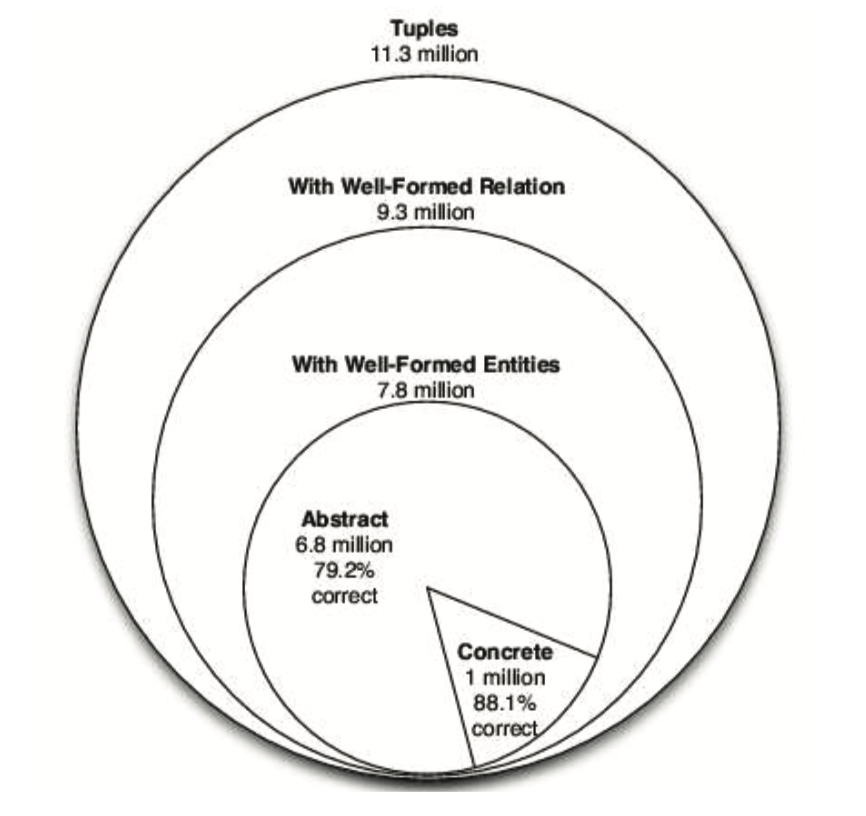
\includegraphics[width=0.5\textwidth]{textrunner.png}
	\caption{TEXTRUNNER在实验环境下知识提取的正确率}
	\label{textrunner}
\end{figure}

Wu等人在TEXTRUNNER的基础上提出了WOE开放信息提取系统\citing{wu2010open}。WOE改进了自监督学习方式用于构建提取器,TEXTRUNNER在提取过程中使用解析器直接从语料库中提取(实体,关系,实体)的三元组数据,而WOE则先从Wikipedia的信息框中提取“属性-值”对,再使用匹配器从文章中找到包含文章主语和“属性-值”对的句子作为语料库中的训练数据。随后测试了两种解析方法的提取器:WOE-parse和WOE-pos,WOE-pos使用和TEXTRUNNER类似的解析方法,根据简单的词性标签,从语料库中的句子解析出(实体,关系,实体)的数据,WOE-parse则选择更复杂的依赖解析树,希望能再复杂长句的解析中得到更好的精确度。

开放信息提取系统会对每个输出的三元组数据给定一个置信度,如果给定一个置信度的下限,高置信度的数据被保留,低置信度的数据被过滤,此时可以通过精确度和召回率测试系统的性能。精确度是指保留的数据中正确的数据所占比例,能反映整体精确度的平均水平。召回率是指保留的数据中正确的数据占所有正确数据的比例,能反映正确的数据在不同置信度的分布情况。

实验分析显示,因为使用了更友好的训练数据,WOE-pos在精确度上更优于TEXTRUNNER,而WOE-parse在解析树的帮助下实现了最好的性能,特别是在召回率上。

Fader等人在分析TEXTRUNNER和WOE的结果之后发现,不连贯提取和无信息提取两种错误频繁出现。不连贯提取是指被提取的关系语句由多词组成,但语义不连贯而无意义。无信息提取是指提取内容忽略了句子的关键信息,例如,“父亲对母亲做出承诺”,系统返回无信息的(父亲,做出,承诺)而不是(父亲,做出承诺对,母亲)。以上的两种错误都是由系统不能提取出具有完整句法结构的关系语句造成的,Fader等人在Open IE系统中引入了一定的句法限制,提出了REVERB开放信息提取系统\citing{fader2011identifying}。30\%的REVERB提取数据的概率标签在0.8或更高,相较起TEXTRUNNER的0.13\%,在精确度上实现了越阶式的增长,不连贯提取和无信息提取的错误率也大幅减少。
\end{comment}

(3)Freebase

Bollacker等人试图结合一般数据库的扩展和Wikipedia等百科全书的多样性,提出了Freebase数据库\citing{bollacker2008freebase}。Freebase和其他常用的知识库相同,使用资源描述框架的三元组形式结构化真实世界的知识,但同时继承了网络百科全书的开放和协同的思想,所有的内容创造和维护都由社区成员协作完成。Freebase存储的元组数据超过1亿2500万条,超过4000种类型和7000种属性,允许使用查询语言通过HTTP协议获取数据。

(4)Wikidata

Wikidata是为了更高效地开放使用和管理Wikipedia文章中数据而提出的协同知识库\citing{vrandevcic2014wikidata}。由于Wikidata的出发点是希望通过大规模协同的方式构建知识库,因此Wikidata的数据具有开放性、多版本共存、多语言、易用性和持续更新的特性。Wikidata向所有用户提供数据扩展和编辑的权限;Wikidata为保证模糊数据的存疑性,相互之间有冲突的数据被同时展示;考虑到数字、日期、坐标等语言无关的数据内容,Wikidata与Wikipedia相同设计为多语言版本;Wikidata数据被组织成Json、RDF的形式发布于网络,通过网络服务能够轻松获取数据;社区成员的持续更新能保持Wikidata的时效性。

Wikidata于2012年提出,相较起以往的知识库,开放性更强,限制也更少。对比YAGO和DBpedia,Wikidata不是从Wikipedia的目录或者信息框中提取信息,相反Wikidata被社区成员独立构建,并为Wikipedia作为知识源,数据被链接到Wikipedia文章中。对比Freebase将对象按类型划分的方式,Wikidata支持对所有对象赋予任意属性。

\section{KBSN模型}
使用RDF的数据表达方式,实体和实体之间通过属性建立了联系,这些有丰富语义的实体之间相互联系,构成了知识库。通过可视化的方式,实体作为节点,属性或者实体关系为边,知识库可以以图的形式呈现,因此知识库也被称为知识图谱。

正如上文中提到的,知识库因其丰富的知识存储量、多样化的知识内容、复杂的知识关联、结构化的数据存储方式,可以作为问答系统或者其他信息检索任务的重要基础。目前使用知识图谱的主流方式是通过SPARQL等结构化查询语言对知识库中的内容进行精准的检索和提取,这种方式人为地建立查询规则、设计相应的知识库存储。

在基于知识库的视觉问答模型中,知识库的使用方式大致分为两种。一种方式为知识库查询类,依照主流的知识库查询的思路,模型提取图片的实体、将实体映射到知识库、转化自然语言为查询语句、查询知识库\citing{wang2015explicit, wang2017fvqa}。这些模型依靠精准的查询语句,对于预先设定好的模板问题能实现优于基线模型的准确率,然而却面临着问题模板设计成本高、数据集难构建、模型泛化能力差等缺点。

另一种方式为联合嵌入类,这种方式不用设计复杂的查询语句,而是将知识库的文本信息转化为额外的特征向量,并联合图像特征和问题特征一起训练。这种方式能省去问题模板和查询语句设计的人工成本,并将模型在更大规模的开放性数据集进行训练。然而,此前的模型却仅仅使用知识库中单个节点的文本信息,例如论文\citing{wu2016ask}根据从图像中预测的属性生成DBpedia查询,得到相关属性的“comment”本文内容,再将这种成段的文本信息转换为固定的特征向量,作为由知识库提供的额外特征与其他两种模态的特征融合。在这种方式中,模型虽然引入了额外的特征,试图提高表征能力,但是这种额外特征仅仅局限于单个节点,因此必然损失了节点互联形成的结构关系,而这种结构关系正是知识库的核心——通过多种关系连接而组织起来的具有丰富语义表征能力的实体网络。

为了利用知识库中关联数据的结构信息,在N-KBSN模型的基础上,本章构建了一个知识库的图嵌入模块,提出了KBSN模型。KBSN模型使用了N-KBSN模型的问题文本和图像特征提取模块、自注意力和引导注意力模块,而在特征融合时引入了知识库的图嵌入。KBSN的基础架构如图\ref{KBSN}。

知识库的图嵌入是KBSN模型有别于其他基于知识库的视觉问答模型的创新之处,其背后的思路为:先从图像和问题文本中识别出核心概念,将核心概念映射为知识库中的核心实体,通过剔除核心实体外无关的实体和链接形成以核心实体为中心的子图,再将各个子图转换为图嵌入,最后子图嵌入融合为图嵌入,以此作为额外特征。
\begin{figure}[H]
	\centering
	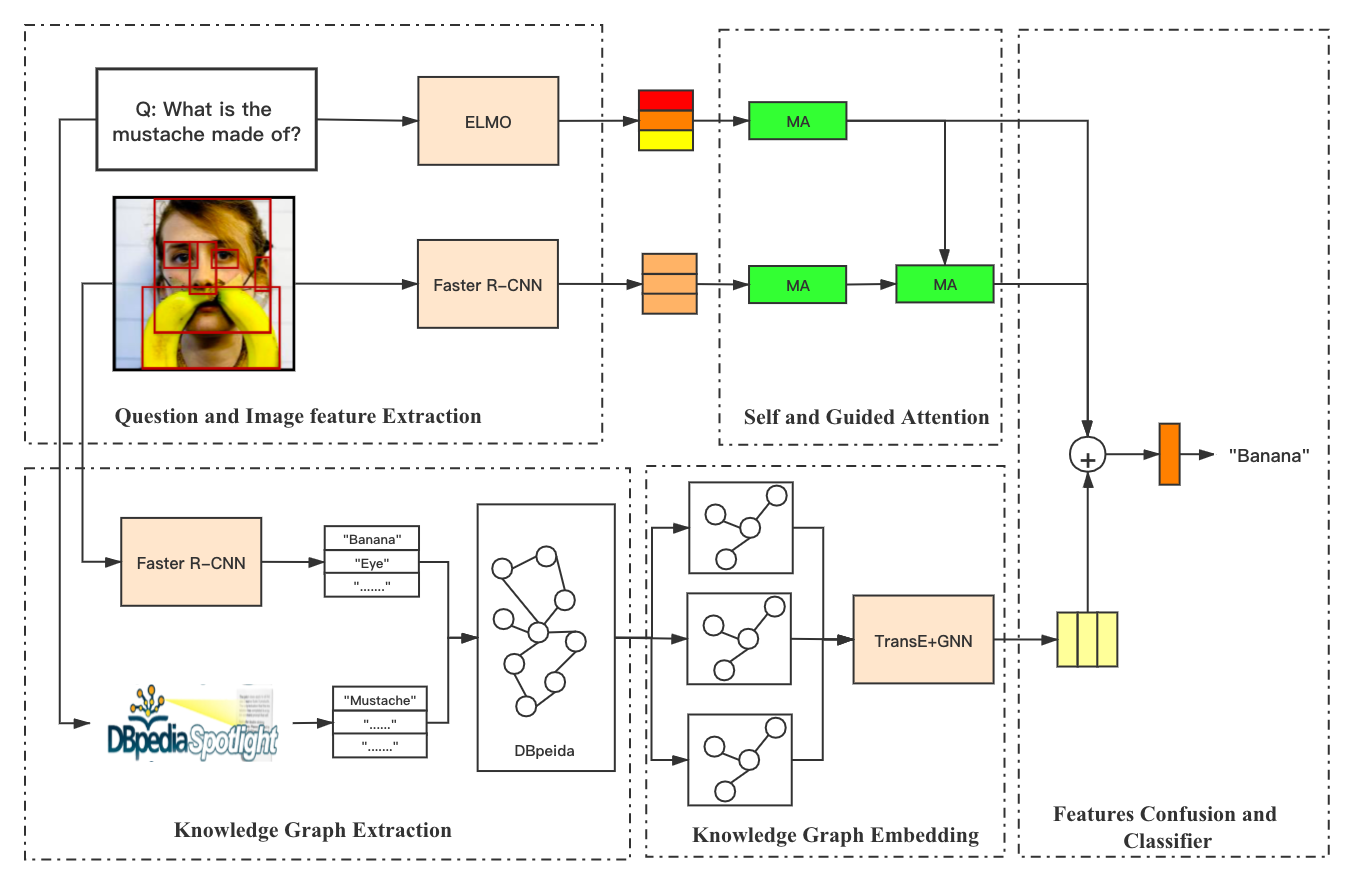
\includegraphics[width=0.8\textwidth]{KBSN.png}
	\caption{KBSN的基础架构}
	\label{KBSN}
\end{figure}

按照以上的思路,知识库的图嵌入由子图提取模块和子图嵌入模块两个主要部分组成。子图提取模块的作用是完成从图像和问题文本到知识库的映射。具体来说,子图提取模块包含“图像-知识库映射”和“文本-知识库映射”。“图像-知识库映射”使用Faster R-CNN预测得到图像中包含的物体,通过查找表,得到图像相关的核心实体;“文本-知识库映射”使用DBpedia Spotlight\citing{isem2013daiber}模型识别、整合问题文本,得到问题相关的核心实体。需要指出的是,在此,本文不是使用完整的DBpedia知识库,而是根据问答这种任务类型的特点,挑选出特定的数据子集构成实验知识库。

子图嵌入模块是将提取得到的子图映射为图嵌入。具体来说,首先使用实验知识库训练TransE模型,得到实验知识库的嵌入表示,然后将子图提取模块输出的子图的节点和边都映射为向量,最后使用向量融合方法获得子图的嵌入表示。最后将子图的嵌入表示、图像特征、文本特征三者融合,分类得到答案,

\subsection{知识库子图提取}
对于基于知识库的视觉问答任务而言,准确的实现自然语言和图像中涉及的实体到知识库实体的映射是至关重要的,一方面能够大大地减少知识库中无关信息的噪声干扰,提高精确度,另一方面准确的映射能够极大的减少计算冗余,提高运行速度。

在知识库子图提取的准确性和计算效率综合的考量下,本文首先以DBpedia为基础,收集了部分子数据集组成实验知识库。再使用在N-KBSN模型中相同的Faster R-CNN从图像中识别出关键实体。另一方面,对于问题文本中的核心实体,模型直接使用DBpedia Spotlight完成从文本到DBpedia节点的映射。在获得图像和文本的核心实体后,模型使用贪婪的子图构建方法,提取出所有以核心实体为主语的三元组,构成知识子图。

需要注意的是,针对图像的物体识别共用的N-KBSN模型中的Faster R-CNN,但是在N-KBSN中,是将所有区域的图像特征融合作为图像特征,而此处则加上分类层,使用softmax预测并输出各个区域的类别信息。由于使用的Faster R-CNN已经在之前的章节详细介绍了,本节将省略面向图像的子图提取,重点介绍面向文本的子图提取。

\subsubsection{面向文本的子图提取}
和基于知识库的问答任务相似,基于知识库的视觉问答任务中的问题文本中并不是每个词语对于答案的得出都起着同等重要的作用。例如对于问题“Is this book writen by Ernest Miller Hemingway”,人类回答者可以忽略句式中的谓语"is"、代词"this",而将句子缩减为(book, writen by, Ernest Miller Hemingway)。这种去除了辅助句法和语法结构的词语而得到的缩减形式便能够反映问题的关键信息,而其中的"book"和"Ernest Miller Hemingway"这类名词在知识库中,被称之为命名实体(named entity),在DBpedia中是以类似于$DBpedia:book$和$DBpedia:Ernest\_Miller\_Hemingway$这种URI的节点形式存在。

对于这些存在于文本中的命名实体的提取便是本小节中面向文本的子图提取的关键步骤之一。而在命名实体的提取中,消除歧义是非常重要的。同一个单词在不同的语境下表达不同的意思,如果不能根据语境正确地判断出单词的特定语义,那么句义的理解就可能偏移,甚至意思完全无法理解。在文本-知识库映射中则体现为,同一个单词子不同语境下对应不同的DBpedia资源,例如"Washington"可以同时对应$DBpedia:George\_Washington$和$DBpedia:Washington,\_D.C$,前者指向“乔治-华盛顿”,一个人,而后者则指向“华盛顿特区”,一个地方,两者的含义千差万别。

为了实现较为准确的命名实体识别,KBSN模型使用DBpedia Spotlight模型\citing{mendes2011dbpedia}实现文本-知识库映射。包括“人物”、“地点”、“组织”这种常见的类别,DBpedia Spotlight能够实现272类DBpedia资源的识别,因此能够很好的识别绝大部分问题中涉及的实体。还可以通过针对数据集的特点使用针对性的配置,进一步提高实体的识别准确率。

DBpedia Spotlight模型主要由三个阶段实现,短语识别阶段从输入的自然语言句子中提取出可能存在DBpedia资源的短语;候选实体筛选阶段将前一阶段得到的一系列短语映射到DBpedia资源,形成候选实体列表;消除歧义阶段根据短语的上下文语境,从候选实体列表中挑选出最佳的DBpedia资源,完成从文本-知识库映射。

短语识别阶段首先通过字符匹配算法从句子中提取词典中包含的短语,再对每个短语自动标注词性,并且去除词性为动词、形容词、副词、介词,剩下的短语作为候选短语。

候选实体筛选阶段根据DBpedia的Disambiguation数据集——包含和特定短语容易混淆的所有其他短语,囊括每一个候选短语的歧义形式的DBpedia资源,例如对于候选短语"Washington",$DBpedia:George\_Washington$和$DBpedia:Washington,\_D.C$都被加入候选实体列表,以便下一阶段的使用。这一阶段实现了由短语到DBpedia资源的映射,并且为了提高结果的准确性,在这一阶段只进行最小化的筛选,尽量多的包含候选实体。

消除歧义阶段使用生成概率模型\citing{han2011generative},根据短语的上下文信息,计算短语和实体匹配的概率,再依照概率阈值得到短语匹配的DBpedia资源,其中短语也称为“实体指称”。假定短语$s$,上下文$c$,每个实体$e$和短语匹配的概率可以根据以下公式得到,
\begin{equation}
P(e,s,c) = P(e)P(s|e)P(c|e)
\end{equation}
其中,$P(e)$表示实体出现的概率,$P(s|e)$表示以短语$s$指代实体$e$的概率,因为多种不同的短语可以指代同一个DBpedia资源,例如短语"Washington"和"George\_Washington"都可以指代$DBpedia:George\_Washington$,$P(c|e)$表示实体在特定语境出现的概率。通过最大似然概率,得到最匹配的实体$e$,即
\begin{equation}
e = argmaxP(e,s,c)
\end{equation}

假定一个包含$M$个实体指称的wikipedia数据集,$P(e)$可以使用以下公式计算,
\begin{equation}
P(e) = \frac{count(e)}{|M|}
\end{equation}
其中$count(e)$表示指向实体$e$的实体指称的数量。$P(s|e)$的公式为,
\begin{equation}
P(s|e) = \frac{count(e,s)}{count(e)}
\end{equation}

对于短语$s$,它的上下文$c$可以使用一个单词窗口来框定,窗口大小设为50。假定上下文$c$包含$n$个单词$t_1t_2...t_n$,那么$P(c|e)$的公式为,
\begin{equation}
P(c|e) = P_e(t_1)P_e(t_2)...P_e(t_n)
\end{equation}
其中$P_e(t)$表示单词$t$出现在实体$e$的上下文的概率,计算公式为,
\begin{equation}
P_e(t) = \lambda P_{e-ML}(t) + (1-\lambda)P_{LM}(t)
\end{equation}
\begin{equation}
P_{e-ML}(t) = \frac{count_e(t)}{\sum_t count_e(t)}
\end{equation}
其中$P_{e-ML}(t)$是$P_e(t)$的最大概率,$P_{LM}(t)$是在wikipedia数据集上计算得到的通用语言模型。

为了防止短语都连接到“空实体”,同样需要计算“空实体”的得分$P(NIL,s,c)$,使用以下公式分别计算$P(NIL)$、$P(s|NIL)$和$P(c|NIL)$,而所有得分小于$P(NIL,s,c)$的实体都会被剔除。
\begin{equation}
P(NIL) = \frac{1}{|M|}
\end{equation}
\begin{equation}
P(s|NIL) = \prod_{t\in S}P_{LM}(t)
\end{equation}
\begin{equation}
P(c|NIL) = \prod_{t\in C}P_{LM}(t)
\end{equation}

在计算得到实体的得分之后,根据得分的高低排序便可以得到最匹配的DBpedia资源,得到核心实体,完成文本-知识库映射。随后,模块从实验知识库中提取出所有以核心实体为主语的三元组,构建出知识子图,完成面向文本的子图提取。

%\subsubsection{面向图像的子图提取}

\subsection{知识库子图嵌入}
在KBSN模型中,从问题文本和图像中提取得到的DBpedia实体被视为核心节点。核心节点从词性的角度看,绝大多数都为名词,从句义的整体来看代表整个句子的核心概念,例如问题“Is there snow on the mountains?”中,模型识别出核心实体$DBpedia:Snow$,并且提取出以Snow为中心的子图。子图中包含大量语义高度相关的属性能作为丰富概念的不同语义层次,例如其属性Subject为$Category:Snow$——表示其分类,属性seeAlso为Blizzard——表示其同义概念。然而图结构的知识子图并不能很好的计算处理,因此本文提出使用分布式表示将知识子图中的实体和关系转化为低维向量。这样做的优点有以下几点:

1)计算的便利性。向量化的节点能够方便的衡量节点的差异和相似度,显著提升计算效率。 

2)实现多模信息的融合。KBSN模型中涉及图像特征、文本特征和知识子图特征三种不同模态的数据结构。知识子图的嵌入能够很好得融合入另外两种特征,这种统一的特征表达方式能够也是适应目前的计算框架——以多维向量为基础的计算方式。

3)便于知识库的扩展。文本使用DBpedia为主要的知识库,然而对于其他主流的知识库,如Freebase,WordNet等,使用的实体和属性名称不尽相同,这会限制模型迁移。而使用分布式表示能够将不同的知识来源映射到同一个语义空间,从而建立统一的表示空间,实现不同知识库的相互适应,提高模型的扩展能力。

多个模型在链路预测任务的实现显示,具有更小参数量的TransE模型能有效的建立实体之间的复杂语义,并且在大规模的知识库上依然有较好的表现,因此文本将使用TransE将知识库子图中的实体和关系转化为向量表示。具体的实验设置和结果分析详见本章的“知识库嵌入实验”。

TransE模型的思路来源于词向量中呈现出的词向量聚集和向量空间的平移不变性。具体来说,在词嵌入空间中具有相似语义的词表示呈现出聚集情况,例如向量$e(German)$和$e(France)$等国家名称距离接近;平移不变性表现为$e(king)-e(queen)\approx e(man)-e(woman)$。前者说明有效的嵌入能够表征词的语义相似性,后者说明向量空间中存在一些固定关系能够连接不同的词嵌入。而在知识库中实体之间是通过显性的关系连接构成一个三元组,这种显性的关系也许能帮助找到一个好的图嵌入方式,使得向量空间中存在和显性关系暗合的隐藏关系,而这种隐藏关系在TransE中被称为“翻译”。

假定E为实体的集合,R为关系的集合,训练集为$S=\{(h,r,t)\}$,其中三元组$(h,r,t)$中h表示“头实体”,$r$表示“关系”,$t$表示“尾实体”,它们的嵌入向量分别用$l_h$、$l_r$、$l_t$表示。TransE希望得到的向量存在以下关系,
\begin{equation}
l_h+l_r \approx l_t
\end{equation}
公式可以看做向量$l_h$经过关系r翻译后得到了$l_t$。

为了学习到符合以上公式的向量,模型使用$d(h+r, t)$计算两个向量的差异度,函数$d$使用L1或者L2距离计算公式。模型的思路为如果对一个正确存在的三元组的$h$或者$t$替换成其他的实体,那么新的差异度$d(h^n,r,t^n)$数值应该尽量大,以体现新三元组的错误性。因此TransE使用以下损失函数,
\begin{equation}
Loss = \sum_{(h,r,t) \in S}\sum_{(h^n,r,t^n)\in S^n}|\gamma+d(h+r, t)-d(h^n,r,t^n)|
\end{equation}

其中,$\gamma$为正确的三元组和错误三元组差异度之间的距离超参数。
\begin{equation}
S^n = {(h^n,r,t)|h^n \in E} \cup {(h^n,l,t)|t^n \in E}
\end{equation}

$S^n$表示替换了头实体或者尾实体的三元组的集合。

% \subsection{基于图神经网络的图嵌入}
% 现实中存在大量可以被转化为图结构的数据,例如化学分子结构、交通网络、知识关联甚至图像,从图结构中挖掘数据关联是图的研究的一个重要领域。在图神经网络被提出以前,传统机器学习处理图的方式主要是通过将图结构转化成形式更简单的数据形式,例如向量\citing{haykin2004comprehensive}。这种图结构简单化的压缩方式损失了图的拓扑结构信息——压缩后的向量不含有节点之间的连接关系,因此缺乏表征能力。为了解决这一问题,Scarselli等人提出了图神经网络(GNN)\citing{scarselli2008graph}。受循环神经网络和马尔科夫链在图结构数据上的应用,GNN统一了两者的优势,使用信息传递机制,不断更新一系列对应图节点的单元,直到节点状态达到稳定的平衡,最后基于这些节点输出结果。由于这种架构能够处理更为广泛的图,例如有向图、无向图、有环图、无环图,成为了近年来新兴的基于统计的图研究方法。

% 受到卷积网络在计算机视觉领域所获巨大成功的激励,近来出现了很多为图数据重新定义卷积概念的方法。这些方法属于图卷积网络(GCN)的范畴。Bruna\citing{bruna2013spectral}等人于2013年提出了关于图卷积网络的第一项重要研究,他们基于谱图论(spectral graph theory)开发了一种图卷积的变体,这种方法直接使用图的拓扑结构,根据图的邻居信息进行信息收集。但是由于基于频谱的模型的计算成本随着图的大小而急剧增加,因此对于大图的计算效率较低,另外这种模型只能使用静态的图,面对动态更新的图时,需要执行全新的计算,因此模型的适应性不好。而基于空间的图卷积网络可以解决上述问题,因此也成为了现在主流的GCN方法。这些方法遵循循环递归邻域聚合(或者消息传递)的模式
% ,其中每个节点聚合其相邻节点的特征向量用于更新当前节点的特征向量,在多轮聚合迭代后,这种聚合了邻居节点信息的特征向量被用来表示该节点。再根据任务的需要决定输出节点层级的特征(node-level)或者图层级的特征(graph-level)。

% 在一般的图中,节点可以表示不同的实体,但是连接节点的边没有区别,都只表示为一种连接关系。然而,知识图谱的边具有语义信息,表示实体之间的特定关系,且不同的边可能具有巨大差异的语义,因此除了节点需要表征为向量,边也需要。假设$G = (V, E)$表示一个图,$X(v_i)$表示节点$i$的节点向量,$v_i \in V $,$X(e_{i,j})$表示节点$v_i, v_j$之间的边向量,$e_{i,j} \in E$。GNN 利用图结构和节点特征 $X(v_i)$ 来学习一个节点的表征向量 $h(v_i)$,或者整个图的表征向量 $h(G)$。遵循领域聚合策略,我们通过聚合它的邻近节点的表征向量来迭代更新节点的表征向量,在第$k$层,
% \begin{equation}
% a_{v_i}^{(k)} = AGGREGATE^{(k)}(Tr(h_{e_j}^{(k-1)}, X(e_{i,j}))), v_j \in N(v_i)
% \end{equation}
% 其中$v_j$为节点$v_i$的邻接节点,$Tr(h_{e_j}^{(k-1)}, X(e_{i,j}))$将上一层的节点的表征向量联合边向量进行融合,$AGGREGATE()$为该层的聚合向量。而$k$层的节点表征向量由下式得到,
% \begin{equation}
% h_{v_i}^{(k)} = COMBINE(h_{v_i}^{(k-1)}, a_{v_i}^{(k)})
% \end{equation}
% 其中,我们初始化$h_{v_i}^{(0)}=X(v_i)$。

% 不同的$AGGREGATE{k}() $和 $COMBINE{k}() $能组合出不同的用于聚合的体系结构,在本文中,我们使用GCN\citing{kipf2016semi}中的方式,将AGGREGATE 和 COMBINE 步集成在一体如下:
% \begin{equation}
% h_{v_i}^{(k)} = ReLU(W*MEAN\{Tr(h_{v_j}^{(k-1)}, X(e_{i,j})), h_{v_i}^{(k-1)}\}), v_j \in N(v_i)
% \end{equation}
% 其中$MEAN\{\}$为element-wise的均值池化。

% 并且为了让知识库中的节点向量能和文本处理模块保持语义的一致性,我们使用elmo初始化节点和边特征,即,
% \begin{equation}
% X(v_i) = elmo(v_i),
% X(e_{i,j}) = elmo(e_{i,j})
% \end{equation}

\section{知识库嵌入实验}
和词嵌入一样,不同的嵌入方式对节点和节点拓扑结构的特征表示能力有差异,而这种差异又会显著影响后续应用,本文中体现为面向视觉问答任务引入的特征的有效性。因此知识库的嵌入方法需要谨慎选择,并且需要证明其有效性。

本节首先对DBpedia进行知识库预处理,得到DBV和DBA两个实验知识库。随后选取了几个在知识库嵌入表现优异的模型进行对比实验,使用知识图谱中的链路预测任务评估知识库嵌入效果。链路预测是通过已知的网络节点及网络结构等信息,预测网络中任意两个节点之间产生连接的可能性。在本文中,链路预测分为训练和测试两个阶段,在训练阶段,模型将高维的知识图谱中的节点和边映射为低维向量,在测试阶段,给定三元组中的头实体和关系(或尾实体和关系)预测尾实体(或头实体),并使用相似性测度衡量模型的差异。

\subsection{知识库预处理}
因为DBpedia丰富的实体及其属性,并且相对规范和统一的数据内容,文文使用DBpedia作为提供额外特征的知识库。如图\ref{KBSN}所展示的基础架构,本文会将知识库的实体和关系转化为低维嵌入表示,再根据问题和图像提取出嵌入的知识库子图,并作为额外特征与图像特征和文本特征融合。为实现知识库的分布式表示,需要需要对原有的DBpedia知识库进行预处理,分别是遴选数据子集、数据清洗、去URI化、创建实验知识库。

(1)遴选数据子集

由于DBpedia从众包的wikipedia提取得到,完整的DBpedia知识库中除了和实体语义高度相关的属性外,还保留着一些语义无关的属性,例如用于连接其他知识库实体的外链、参考引用的外链、主页地址、图片链接、未经处理的infobox属性等,除此之外,完整数据集中还包含包括英语在内的多语言版本。而以上这些信息对于回答开放性问题帮助很小,因此本文首先从DBpedia中遴选出“包含丰富语义”的子数据集,具体的数据集及其简要描述如表\ref{dbpeidaList}。
\begin{table}[H]
% \resizebox{0.8\textwidth}{!}{}
\centering
\caption{遴选的DBpedia数据子集及其描述}
\begin{adjustbox}{max width=0.8\textwidth}
\begin{tabular}{lc}
\toprule
DBpedia数据集 & 描述\\
\midrule
instance\_types\_en & 连接实体及其类型 \\
labels\_en & 实体标签 \\
mappingbased\_literals\_en & 连接object为literal的高质量的谓语 \\
mappingbased\_objects\_en & 连接object为对象的高质量的谓语 \\
persondata\_en & 和person相关的信息,例如出生日期等 \\
\bottomrule
\end{tabular}
\end{adjustbox}
\label{dbpeidaList}
\end{table}

正如表\ref{dbpeidaList}所示,本文只选取了英语版本的知识库,但值得注意的是,本文提出的模型结构同样适用于其他语言类型,扩展到多语言的应用只需要将数据集和知识库替换为指定语言版本即可。遴选的知识库子集包含完整的类别信息、完整的实体标签和高质量的属性信息,足够应对绝大部分的常规问题,例如VQA2.0数据集中涉及的对象和属性都存在于实验知识库中。


(2)数据清洗

在选定知识库子集后,本文使用virtuoso opensource将知识库子集加载成一个命名图(http://dbpedia.org),并使用本地服务器提供SPARQL应用交互接口,并分析了其数据内容,如表\ref{dbpediaPara}所示。
\begin{table}[H]
% \resizebox{0.8\textwidth}{!}{}
\centering
\caption{知识库子集的参数统计}
\begin{tabular}{lc}
\toprule
统计参数 & 数量\\
\midrule
三元组 &  59,998,758\\
类 &  426\\
实体 & 5,377,081 \\
主语 & 14,556,042 \\
谓语 & 1,377 \\
宾语 & 19,495,719 \\
\bottomrule
\end{tabular}
\label{dbpediaPara}
\end{table}

如表所示,知识库子集中三元组数量接近6000万,数据量非常庞大。一方面,庞大的数据量能覆盖更加广泛的知识内容,这蕴含着提高视觉问答准确性的更大的可能性,但另一方面,知识库的所有实体和关系都需要嵌入到同一个特征空间,数据量越大,特征向量计算难度越大,特征化的效果难以保证。因此本文进一步研究了数据内容的特征,进一步清洗数据。

表\ref{dbpediasamples}展示了一条知识库中的三元组数据,和实例相同,在DBpedia中,以“http://dbpedia.org/resource/ResourceName”的URI形式存在的节点被称为“资源”。“资源”是DBpedia的核心节点,可能出现在三元组的主语或者宾语。本文的知识库提取模块也是分别从图像和文本中提取DBpedia“资源”,因此“资源”是本文首要关注的节点。

\begin{table}[H]
% \resizebox{0.8\textwidth}{!}{}
\centering
\caption{知识库子集的三元组实例}
\begin{tabular}{lll}
\toprule
主语 & <http://dbpedia.org/resource/Snow> \\
谓语 & <http://www.w3.org/1999/02/22-rdf-syntax-ns\#type> \\
宾语 & <http://www.w3.org/2002/07/owl\#Thing>\\
\bottomrule
\end{tabular}
\label{dbpediasamples}
\end{table}

为了方便后续的数据清洗,本文首先提取了所有三元组的中包含的DBpedia资源,建立了一个资源序列表。资源序列表中包含知识库中接近1500万个DBpedia资源。本文使用SPARQL批量查询了各个资源的谓语数量,得到如表\ref{predicateNum}所示的统计信息。

\begin{table}[H]
% \resizebox{0.8\textwidth}{!}{}
\centering
\caption{DBpedia资源的谓语数量}
\begin{tabular}{cccc}
\toprule
谓语数量范围 & 谓语数=0 & 谓语数=1 & 谓语数>1\\
\midrule
$[0, 37]$ &  391,904 &  9,190,505 & 5,365,537\\
\bottomrule
\end{tabular}
\label{predicateNum}
\end{table}

如表\ref{predicateNum}所示,数据集中DBpedia资源的谓语数量最小为0,最大为37。谓语数量为0的资源有将近40万,这类资源在三元组中充当宾语。谓语数量为1的资源有900万左右,所有这些资源的谓语都是“<http://www.w3.org/2000/01/rdf-schema\#label>”,宾语都是各自的英文名称,除此以外知识库中不包含任何其他的属性。以上两种资源都对于本次研究没有意义,因为这些资源在知识库中没有其他有价值的属性,因此不能为模型提供额外的信息。所以本文剔除了包含以上两种DBpedia资源的三元组,保留了所有剩余的三元组。

(3)去URI化

正如表\ref{dbpediasamples}所展示的,DBpedia的实体多是以URI的形式表示的,这种表示方式的优势是DBpedia资源直接对应一个网络资源,可以通过浏览器直接访问相应节点,方便构建和其他数字资源的关系。然而在本文的研究中,并不会使用到这种特性,反而因为表示网站地址的前缀和节点的语义并无联系,冗余的表示方法不仅增大了文本存储的空间,也降低了本文匹配的效率。

因此我们研究了实体和属性的表示方法,将所有节点去URI化,去除后的结果实例如表\ref{deuri}。
\begin{table}[H]
% \resizebox{0.8\textwidth}{!}{}
\centering
\caption{节点去URI化的实例}
\begin{adjustbox}{max width=0.8\textwidth}
\begin{tabular}{cccc}
\toprule
 & 去URI前 & 去URI后\\
\midrule
主语 &  <http://dbpedia.org/resource/Snow> &  Snow \\
谓语 & <http://www.w3.org/1999/02/22-rdf-syntax-ns\#type>  & 22-rdf-syntax-ns\#type \\
宾语 & <http://www.w3.org/2002/07/owl\#Thing> & owl\#Thing\\
\bottomrule
\end{tabular}
\end{adjustbox}
\label{deuri}
\end{table}

(4)创建实验知识库

为研究知识库大小对模型的影响,本文创建了两个实验数据库:DBV和DBA。DBA知识库是经过以上的处理步骤得到的完整知识库;DBV知识库是根据特定规则从DBA知识库提取得到的,规则为三元组均以VQA2.0数据集的问题所包含的DBpedia资源为主语。两个知识库的统计信息如表\ref{DBV-DBA}。
\begin{table}[H]
% \resizebox{0.8\textwidth}{!}{}
\centering
\caption{DBV和DBA知识库的统计信息}
\begin{tabular}{ccc}
\toprule
统计量 & DBV & DBA \\
\midrule
三元组数 & 98,201 & 52,247,554 \\
主语数 &  7,863 &  5,365,537 \\
谓语数 & 1,377 & 1,377 \\
\bottomrule
\end{tabular}
\label{DBV-DBA}
\end{table}

如表\ref{DBV-DBA}所示,DBV和DBA知识库均包含了1377个谓语,这和数据清洗前的知识库相同。数据清洗后,DBA知识库的三元组数比初始的知识库少了700万,占比为13\%,这明显得减少了数据冗余,说明数据清洗的必要性。DBV知识库包含了7800个主语,9万个三元组,虽然其数量远小于DBA知识库,但是该知识库的三元组的主语与VQA2.0数据集中的问题高度相关,本文构建该知识库去测试其在视觉问答任务的表现。

\subsection{模型选择和对比}
本文选取了几个在知识库嵌入表现优异的模型作为测试模型,包括结构化嵌入(SE)\citing{bordes2014semantic}、语义匹配能量函数(SME)\citing{bordes2011learning}、TransE模型\citing{bordes2013translating}。TransE模型已经在前文中详细介绍了,其主要思想为将知识库中的实体和关系都嵌入为一个低维向量,对于一个存在的三元组$(h, r, t)$,$d(l_h+l_r, l_t)$应该更小,相比于不在同一个三元组的两个实体而言。类似的,SE仍然使用向量的距离度量实体是否在同一个三元组。不过在SE中,关系被嵌入为两个关系矩阵$R_k^h\in \mathbb{R}^{k \times k}, R_k^t \in \mathbb{R}^{k \times k}$,并且使用$d(R_k^hh, R_k^tt)$度量两个实体的距离。SME先将知识库的实体和关系转化为向量,再使用神经网络去训练一个语义匹配能量函数$\varepsilon((h,r,t))$,使得处于同一个三元组的两个实体的能量最低,从而实现链路预测。SME又根据使用的函数不同分为SME(LINEAR)和SME(BILINEAR)。

虽然以上的模型背后的思想都是以关系为基准度量两个实体之间的距离,从而实现头实体和尾实体的匹配,进而完成链路预测。但是其实现方法的不同导致模型的参数数量不同,表\ref{model_compar}对比了四种模型的参数量和在FB15K、DBV、DBA上的具体参数量。
\begin{table}[H]
% \resizebox{0.8\textwidth}{!}{}
\centering
\caption{不同知识库嵌入模型的理论参数量和实际参数量(百万)}
\begin{tabular}{lllll}
\toprule
模型 & 理论参数量 & FB15K(M) & DBV(M) & DBA(M) \\
\midrule
SE & $O(n_ek + 2n_rk^2)$ & 7.47 &  7.14 & 434.93\\
SME(LINEAR) & $O(n_ek + n_rk + 4k^2)$ &  0.82 &  2.82 & 428.54 \\
SME(BILINEAR) & $O(n_ek + n_rk + 2k^3)$ & 1.06 & 3.06 & 428.78 \\
\midrule
TransE & $O(n_ek + n_rk)$ & \textbf{0.81} & \textbf{2.81} & \textbf{428.53}\\
\bottomrule
\end{tabular}
\label{model_compar}
\end{table}
其中$n_e, n_r$分别表示数据集中实体和关系的数量,$k$表示嵌入的维度,在计算具体值时,设定$k=50$。从表中可以看出,随着数据集中的实体和关系数量的增加,所有模型的参数量都逐步增加,其中SE模型对关系数量相较其他三个模型更为敏感。总体来看,TransE具有参数较少的优点,在任意大小的数据集上,其参数量均为最少。SME(LINEAR)、SME(BILINEAR)和TransE的参数量接近,其差距主要取决于向量的维度,TransE更容易实现更高维度的嵌入。

\subsection{实验设置}

1)数据集。为了测试模型在不同体量的知识库上的表现,本文使用三个数据量差异明显的数据集——FB15K、DBV和DBA。FB15K从Freebase中筛选和提取得到的,数据包含592213条三元组,涉及14951个实体和1345种关系。DBV和DBA是本文提出的从DBpedia提取得到的两个知识库数据集,其中DBV数据集中的三元组数据的主语提取自VQA2.0数据集的问题文本,是本文专门设计的面向视觉问答任务的数据集,其包含98201条三元组数据,涉及55341个实体和874种关系。DBA包含5200万条三元组数据,涉及856万个实体和1293种关系。三个数据集的统计信息如表\ref{3kb}所示。
\begin{table}[H]
% \resizebox{0.8\textwidth}{!}{}
\centering
\caption{FB15K、DBV和DBA数据集的统计对比}
\begin{tabular}{llll}
\toprule
统计量 & FB15K & DBV & DBA \\
\midrule
三元组数 & 592,213 & 98,201 & 52,247,554 \\
实体数 & 14,951 &  55,341 &  8,569,361 \\
关系数 & 1,345 & 874 & 1,293 \\
训练集三元组数 & 483,142 & 80,200 & 41,798,043\\
验证集三元组数 & 50,000 & 9,000 & 5,224,755\\
测试集三元组数 & 59,071 & 9,001 & 5,224,756\\
\bottomrule
\end{tabular}
\label{3kb}
\end{table}

从数据量的角度分析,DBA数据集的三元组数和实体数均高出其他两个数据集两个数量级,而这样大体量的数据集一方面更接近真实场景的知识量,另一方面要求模型具有很好的尺度变化能力。DBV数据集的实体数是FB15K的3.7倍,但是数据量仅为FB15K的1/7,这说明DBV数据集中的单个头实体对应的平均尾实体数少于FB15K,这种特性理论上能实现更易区分的特征向量。

数据集按照$8:1:1$的比例被划分为训练集、验证集合测试集,并且保证了测试集中的节点均在训练集或验证集中出现。

2)实验评估。为了评估模型的表示学习的效果,实验使用排名相关的评估标准。具体来说,对于每一个测试三元组,首先先将头实体替换成数据集中其他的实体,组成新的三元组,并通过模型计算得到其差异值或者能量。基于模型的假设,正确的三元组应该具有更低的能量或者差异值,因此对每一个新构成的三元组的差异值或者能量按照从低到高的升序排序,进而得到正确的实体的排名。再对测试三元组进行替换尾实体的操作,并再次计算正确实体的排名,重复直到所有测试三元组均完成了头实体和尾实体的替换。最后将所有正确实体的排名取均值,得到的Mean Rank作为一个评估指标。另一个评估标准为正确实体排名前十的比例——hits@10。

3)参数设置。本节实验的四个模型均使用梯度下降算法更新参数,选取学习率的范围$\lambda \in \{0.001,0.01,0.1\}$,特征向量的维度$k \in \{20,50\}$,向量的距离计算使用$L_1$或者$L_2$距离计算公式,TransE中使用的距离超参数$\gamma \in \{0.5, 1, 2\}$。训练代数最多为1000代,并且根据验证集的Mean Rank保存最优模型的参数和状态。

其中TransE针对FB15K、DBV、DBA数据集上的最佳参数配置如表\ref{optimal_config}所示。
\begin{table}[H]
% \resizebox{0.8\textwidth}{!}{}
\centering
\caption{TransE对FB15K、DBV和DBA数据集的最佳参数}
\begin{tabular}{llll}
\toprule
参数 & FB15K & DBV & DBA \\
\midrule
特征向量维度$k$ & 50 & 50 & 50 \\
学习率$\lambda$ & 0.01 &  0.01 &  0.01 \\
距离参数$\gamma$ & 0.5 & 1 & 1 \\
距离计算式$d$ & $L_2$ & $L_1$ & $L_1$\\
\bottomrule
\end{tabular}
\label{optimal_config}
\end{table}

\subsection{实验结果及分析}
实验结果如表\ref{results}所示。从每个数据集的结果来看,TransE的Mean Rank和hits@10均优于其他三个模型。具体来说,在FB15K数据集上,TransE的Mean Rank最低,且优于其他三个模型80左右,而在hits@10的准确率上更是高出10\%左右,大幅领先于其他三个模型。这一整体的领先也体现在DBV数据集上,并且随着数据量的增加,TransE的优势继续扩大。
\begin{table}[H]
% \resizebox{0.8\textwidth}{!}{}
\centering
\caption{四个模型在链路预测任务的实验结果}
\begin{adjustbox}{max width=\textwidth}
\begin{tabular}{lcccccc}
\toprule
数据集 & \multicolumn{2}{c}{FB15K} & \multicolumn{2}{c}{DBV} & \multicolumn{2}{c}{DBA} \\
\midrule
评估标准 & Mean Rank & hits@10(\%) & Mean Rank & hits@10(\%) & Mean Rank & hits@10(\%) \\
\midrule
SE & 273 & 28.8 & 1043 & 48.5 &  604836 & 35.4\\
SME(LINEAR) & 274 & 30.7 &  1057 & 51.4 & 618265 & 37.2 \\
SME(BILINEAR) & 284 & 31.3 &  1150 & 53.1 & 634921 & 42.6 \\
\midrule
TransE & \textbf{195} & \textbf{41.2} &  \textbf{817} & \textbf{67.6} & \textbf{567420} & \textbf{54.6} \\
\bottomrule
\end{tabular}
\end{adjustbox}
\label{results}
\end{table}
根据不同数据集的结果可以得知,随着数据集的体量的增加,待嵌入的节点数增加,模型的Mean Rank呈现下降趋势,其中SE、SME(LINEAR)和SME(BILINEAR)的升高尤其明显,TransE在面对大数据集时,性能下降平缓,这是由于其模型的简洁性带来的扩展性能的提升。值得注意的是,四个模型在DBA的实验结果均明显差于DBV,并且其Mean Rank非常高,大于50万,而且模型在DBA数据集上的单次训练时间是DBV的数百倍。这说明DBA知识库虽然包含有更多的数据,理论上能实现更精准的嵌入,但是碍于算力和模型的精度,其并没有很高的实用性。

但是对比DBV和FB15K上hits@10指标,结果的趋势和Mean Rank并不相同。DBV数据集待嵌入的节点数是FB15K的3.7倍,但是可用于训练的三元组仅仅是FB15K的1/7,但是其hits@10准确率却更高,TransE在DBV上的准确率比在FB15K上高出26.4\%,同样的情况发生在其他三个模型上。

为了进一步理解模型在Mean Rank和hits@10两种指标上呈现出的不同趋势,本文将FB15K和DBV三元组中的关系类型分成了四种类型:一对一、一对多、多对一、多对多。一对一的关系类型的头实体和尾实体一一对应,一对多的关系的每一个头实体对应多个尾实体,多对一的关系的尾实体对应多个头实体,多对多的关系则是多个头实体和多个尾实体对应。具体来说,对于关系$r$,在数据集中,累加其每个尾实体对应的头实体数得到总的头实体数,再除以尾实体个数,得到平均头实体数,同理可以得到平均尾实体数。如果平均头实体数小于1.5,且平均头实体数小于1.5,则关系划分为一对一,同理可得其他三种关系,如表\ref{rel_type}所示。
\begin{table}[H]
% \resizebox{0.8\textwidth}{!}{}
\centering
\caption{四种关系类型的划分标准}
\begin{tabular}{ccc}
\toprule
关系类型 & 平均头实体数 & 平均尾实体数 \\
\midrule
一对一 & < 1.5 & < 1.5 \\
一对多 & < 1.5 & >= 1.5 \\
多对一 & >= 1.5 & < 1.5 \\
多对多 & >= 1.5 & >= 1.5 \\
\bottomrule
\end{tabular}
\label{rel_type}
\end{table}

根据上表的划分标准,本文分析了FB15K和DBV中关系类型的分布,如表\ref{rel_dist}所示。FB15K数据集中四种类型分布较为均匀,而DBV数据集中一对一的关系占比超过50\%,为主要类型。一对一的关系所在的三元组中,头实体和尾实体的对应关系相对清晰,可能更利于模型训练更易区分的特征表示。
\begin{table}[H]
% \resizebox{0.8\textwidth}{!}{}
\centering
\caption{FB15K和DBV中关系类型的分布}
\begin{tabular}{ccc}
\toprule
占比(\%) & FB15K & DBV \\
\midrule
一对一 & 26.2 & 50.2 \\
一对多 & 22.7 & 11.1 \\
多对一 & 28.3 & 26.8 \\
多对多 & 22.8 & 11.9 \\
\bottomrule
\end{tabular}
\label{rel_dist}
\end{table}

为了分析不同关系类型和准确率的关系,本文分析了TransE模型在FB15K和DBV数据集上,对于四种关系类型的hits@10的准确率,如表\ref{rel_hits10}所示。
\begin{table}[H]
% \resizebox{0.8\textwidth}{!}{}
\centering
\caption{TransE在FB15K和DBV数据集的结果对比}
\begin{tabular}{ccccccccc}
\toprule
任务 & \multicolumn{4}{c}{预测头实体hits@10(\%)} & \multicolumn{4}{c}{预测尾实体hits@10(\%)} \\
\midrule
关系类型 & 一对一 & 一对多 & 多对一 & 多对多 & 一对一 & 一对多 & 多对一 & 多对多\\
\midrule
FB15K & 43.7 & 65.7 & 18.2 & \textbf{47.2} & 43.7 & 19.7 & 66.7 & 50.0\\
DBV   & \textbf{81.8} & \textbf{81.7} & \textbf{32.8} & 47.0 & \textbf{83.2} & \textbf{75.9} & \textbf{74.6} & \textbf{58.8}\\
\bottomrule
\end{tabular}
\label{rel_hits10}
\end{table}

如上表所示,无论是预测头实体还是尾实体,TransE在DBV数据集上,基本上对于所有的关系类型的hits@10均高于其在FB15K的表现,其中对于一对一的关系的hits@10的准确率两倍于FB15K的表现,其他类型也有明显的提升,这显示了TransE在DBV整体hits@10指标上优于FB15K的原因。

四种关系类型的准确率差异显示,无论是在哪个数据集,TransE在预测实体数为一的一边时,具有更高的准确率,例如,在预测头实体任务中,“一对一”和“一对多”的准确率高于其他各种类型,而在预测尾实体任务中,“一对一”和“多对一”的准确率高于“一对多”和“多对多”的类型。这说明TransE模型更适合处理“一一映射“的数据。

TransE对DBV数据集中一对一的关系,预测准确率达到81.8\%和83.2\%,表现出极高的预测准确率。高准确率证明了TransE模型的节点嵌入的有效性。对于一对一的关系类型,头实体和尾实体存在一一对应关系,而无关节点则应当充分远离。高hits@10说明模型能够有效区分正确的匹配和错误的匹配,实现无关节点的距离最远。此外,TransE之所以在DBV上有更优的表现,这说明DBV中三元组的实体之间对应性更强,更便于节点的嵌入。表\ref{rel_dist}印证了该结论。

\textbf{结论}\qquad
SE、SME(LINEAR)、SME(BILINEAR)和TransE在链路预测上的实验证明,TransE模型在参数更少的情况下,具有更好的节点嵌入表现,且面对不同体量的知识库时,其在尺度扩展的能力也是最优,因此非常适合用于大知识库的节点嵌入。

通过对TransE在FB15K和DBV数据集上更细粒度的实验,结果显示TransE模型能够非常有效的编码节点,对于存在一一对应关系的实体,其预测准确率尤其高。此外,DBV数据集中的实体之间的对应性更强。在训练数据较少并且待嵌入节点数更多的情况下,同样的模型能实现更高的链路预测的准确率,即更优的节点嵌入表示。因此DBV数据集优于FB15K。

另一方面,虽然DBA数据集相较于DBV拥有更多的数据和实体,但实验结果证明,巨大的数据量成为了知识库嵌入训练的障碍,四个实验模型在DBV数据集上的hits@10也远高于DBA。结果说明DBA对于目前的模型而言,并没有太大的实用价值,因此此后的视觉问答任务实验仅仅使用构建的DBV知识库。

\section{视觉问答任务实验}
本节实验将使用使用多个数据集训练和评估本文构建的基于知识库图嵌入的视觉问答模型(KBSN)。为了验证知识库图嵌入对结果的影响,实验还构建了一系列对比模型,包括上一章提出的$N-KBSN(l)$。整体代码使用Python实现,以pytorch为机器学习平台,并使用带有32G内存和GPU的计算机训练模型。

\subsection{实验设置}
(1)参数设置

本章提出的KBSN模型是在上一章提出的N-KBSN模型的基础上,引入了知识库子图提取模块和子图嵌入模块后构建而成。因此图像和文本提取模块、注意力机制、特征融合和分类器的参数配置都和$N-KBSN(l)$相同。其中Elmo模型的双向长短期网络(biLSTM)隐藏层维度为4096,单层输出维度为512,Elmo动态词向量维度为1024。

知识库子图提取模块使用了和图像特征提取模块中相同的Faster R-CNN网络。不同之处在于,图像特征提取仅仅使用兴趣区域的特征,而知识库子图提取模块添加了两个全连接层和softmax层用于预测图像中的物体,其中,单张图像被检测对象数量$m\in [5, 10]$分类器的大小为1600。Spotlight模型的单词窗口大小设为50。

(2)数据集

由于KBSN模型引入的外源知识库能一定程度增强模型对先验问题的感知,因此实验除了使用VQA2.0数据集\citing{goyal2017making}外,还使用了KB-VQA数据集\citing{wang2015explicit}。KB-VQA包含700张图片,150个物体类别和100个场景类别,总共包含2741个问答对。问题类型包含“常识问题”、“视觉问题”和“知识库”问题,它们各自的数量为1256、883、263。依照第三章的数据集划分,VQA2.0被划分为train/val/test,比例为2:1:2。由于KB-VQA中的图片全部包含于VQA2.0中,并且考虑到其数据量较小,因此KB-VQA数据集仅分为train/test,比例为1:1。

(3)知识库

本节将使用上文构建的提取自DBpedia的知识库:DBV。DBV中三元组的主语均提取自VQA2.0数据集中的问题,包含98201条三元组。

(4)评估方式

基于VQA2.0数据集的实验的评估方式详见第三章实验评估部分。KB-VQA的评估方式也使用人工标注,具体来说,测试者评估答案的正确性,并且给出五个分数,1:完全错误;2:些许错误;3:及格;4:正确;5:完全正确。得分大于三分的答案被判定为正确,否则为错误。

实验结果均使用正确率为指标,其中VQA2.0的实验结果包括总体正确率、是否问题正确率、计数问题正确率和其他问题正确率,KB-VQA实验结果包括总体正确率、视觉问题正确率、常识问题正确率和知识库问题正确率。

\subsection{实验结果分析}
\subsubsection{VQA实验结果分析}
本小节使用VQA2.0数据集进行实验,参与实验的模型有$N-KBSN(l)$、$KBSN(spotlight)$、$KBSN(rcnn)$、$KBSN$。其中,$N-KBSN(l)$为前文构建的基于动态词的联合嵌入模型,$KBSN(spotlight)$和$KBSN(rcnn)$分别为在$N-KBSN(l)$基础上添加文本子图提取和图像子图提取的对照模型,$KBSN$为在$N-KBSN(l)$基础上同时引入图像子图提取和文本子图提取的视觉问答模型。各个模型在val验证集上的实验结果如表\ref{4modelres},结果包括总体正确率以及三种答案类型:是否、计数、其他的单项正确率。
\begin{table}[H]
% \resizebox{0.8\textwidth}{!}{}
\centering
\caption{使用不同子图提取模块的模型在val数据集的结果}
\begin{tabular}{ccccc}
\toprule
模型 & 总体正确率 & 是否 & 计数 & 其他\\
\midrule
$N-KBSN$& 67.72 & 85.22 & 49.63 & 59.20\\
\midrule
$KBSN(spotlight)$&  67.76& 85.26&  49.64& 59.25\\
$KBSN(rcnn)$&  67.95& 85.53&  50.04& 59.31\\
$KBSN$&  \textbf{68.04}& \textbf{85.61}&  \textbf{50.23}& \textbf{59.40}\\
\bottomrule
\end{tabular}
\label{4modelres}
\end{table}

如表所示,本章提出的基于知识库图嵌入的视觉问答模型$KBSN$及其两个变体在各项结果的准确率上均高于$N-KBSN$模型,但不同变体的提升幅度有着明显差异。具体来说,仅加入文本子图提取的$KBSN(spotlight)$相较于$N-KBSN$仅仅只有0.05个百分比的提升,而加入图像子图提取的$KBSN(rcnn)$则有将近2个百分点的提高,这种差异也同时体现在三个子项的准确率上。可能的原因有两点:第一,VQA2.0中的问题长度普遍较短,因此能提取得到的实体数量较少。第二,图像相较于问题文本具有更丰富的语义,图像子图提取能够获得更多和答案紧密相关的信息,因此对于最终结果的提升作用更大。

计数问题对图像识别的准确率的较高要求,因此计数问题能体现模型对图像中对象的感知能力。在计数问题的准确率上,$KBSN(rcnn)$相比于$N-KBSN$提升了0.41\%,而$KBSN(spotlight)$仅提升了0.01\%,这说明图像子图提取模块的确增强了模型对图像的解析能力。

$KBSN$因为同时添加了两个模块,结果是四个模型中最优的,但是准确率的提升并不明显。

\subsubsection{KB-VQA实验结果分析}
相较于VQA2.0数据集,KB-VQA数据集的体量更小,但是其问题中除了包含“视觉问题”外,还包含需要复杂推理或者外源知识的“常识问题”和“知识库问题”,因此对模型的推理能力要求极高。本小节仍然使用$N-KBSN(l)$、$KBSN(spotlight)$、$KBSN(rcnn)$、$KBSN$四个模型进行对比实验。

首先将四个模型在VQA2.0训练集上完成预训练,再使用KB-VQA的训练集进行迁移训练,最后使用KB-VQA的测试集评估模型。实验结果中引用了Ahab模型的结果,Ahab模型专门针对KB-VQA数据集的问题,人工构建了知识库查询语句,属于知识库查询类模型。实验模型在KB-VQA测试集上的实验结果如表\ref{kbvqares},结果的直方统计图如图\ref{kbvqagraph}。如图表所示,$N-KBSN$在所有模型中表现最差,由于该模型没有引入任何知识库的嵌入,其推理信息仅仅来源于训练集中的图像和文本,因此其在视觉问题的正确率远远高于常识问题。知识库问题表现极差,正确率仅有17.4\%。
\begin{table}[H]
% \resizebox{0.8\textwidth}{!}{}
\centering
\caption{实验模型在KB-VQA测试集上的结果}
\begin{tabular}{ccccc}
\toprule
模型 & 总体正确率 & 视觉问题 & 常识问题 & 知识库问题\\
\midrule
$N-KBSN(l)$& 37.5 & 47.8 & 33.5 & 17.4\\
\midrule
$KBSN(spotlight)$&  42.8& 49.4&  37.3& 30.3\\
$KBSN(rcnn)$&  47.3& 53.0&  42.3& 37.1\\
$KBSN$&  53.7& 56.7&  50.5& 46.2\\
\midrule
$Ahab$&  \textbf{69.6}& \textbf{67.2}&  \textbf{70.1}& \textbf{75.0}\\
\bottomrule
\end{tabular}
\label{kbvqares}
\end{table}

\begin{figure}[H]
	\centering
	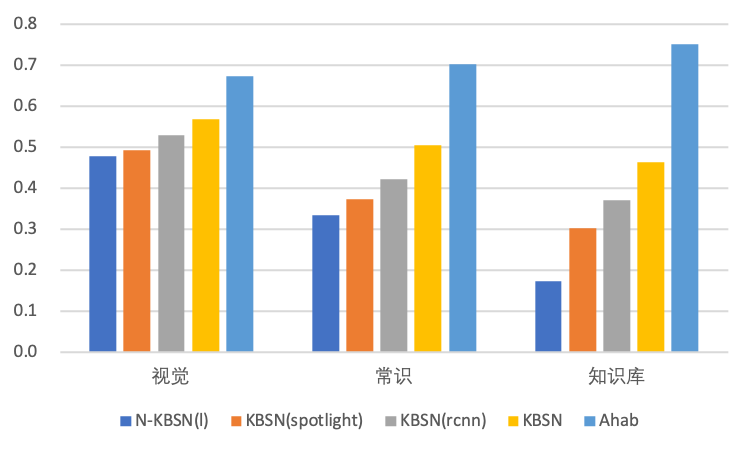
\includegraphics[width=0.8\textwidth]{kbvqagraph.png}
	\caption{不同模型在不同问题类型的准确率}
	\label{kbvqagraph}
\end{figure}

从知识库问题的正确率来看,$KBSN(spotlight)$和$KBSN(rcnn)$由于都部分引入了知识库中的节点,所以正确率相较$N-KBSN$大幅提高,这说明无论是文本子图嵌入还是图像子图嵌入均能一定程度的提高模型对知识库问题的解决能力。从视觉问题的准确率看,前四个模型的准确率差距较小,这说明作为基础模型的$N-KBSN$擅长于解决视觉问题,这和其在VQA2.0数据集上的优秀表现有关。所有模型在常识问题的准确率均介于视觉问题和知识库问题之间,这说明三类问题的难度梯度非常明显,表现为知识库问题 > 常识问题 > 视觉问题。

本文构建的$KBSN$相较于前三个模型,准确率全面领先,这说明文本子图提取和图像子图提取是互补的,每新增一个模块都能提升准确率。

$Ahab$在各项内容的准确率上均呈现出大幅的领先,这是因为其针对KB-VQA数据集中的每一种问题类型均设计了相应的SPAQL查询语句,使其能够精准的查询得到知识库的节点。实验结果也证明了,在推理能力上,知识库查询类模型($Ahab$) > 知识库嵌入类模型($KBSN$) > 联合嵌入模型($N-KBSN(l)$)。

\subsubsection{子图提取模块分析}
根据以上两个在VQA2.0和KB-VQA数据集的实验可以看出,引入了知识库图嵌入的KBSN模型相较于N-KBSN模型的准确率提升在不同数据集上的效果差距明显。具体来说,在VQA2.0数据集上,KBSN的总体正确率仅提升了0.42\%,而在KB-VQA数据集上,提升了16.2\%。为了探究其准确率提升的差异性,本节探究了子图提取模块在两个数据集上的实际表现。

为了衡量子图提取模块的作用,本文提出了子图参与率$jr$和子图准确率$jc$两个指标。具体来说,子图参与率是指知识库子图提取模块有效的从问题文本中提取出了核心实体比例。值得注意的是,定义里并不考虑从图像中提取子图,这是因为模型能从所有样本的图像中识别物体,从而构成子图,但是问题文本可能由于太简单而不包含DBpedia实体。子图准确率是指针对提取出子图的问题,模型的答案准确率。

% 假定KBSN和N-KBSN的准确率差为$\Delta$,在理想情况下,即准确率的提升完全来源于知识库的引入,则满足下式,
% \begin{equation}
% \Delta = jr * jc
% \end{equation}
% 我们使用$\Delta^0$表示实际准确率差。

实验数据来自于$KBSN$在两个数据集上的结果,结果详见表\ref{kbsn_compr},双饼图见图\ref{kbsn_graph},左边的饼状图表示子图参与率,右边饼状图表示子图准确率。
\begin{figure}[H]
	\centering
	\subfigure[VQA2.0]{
		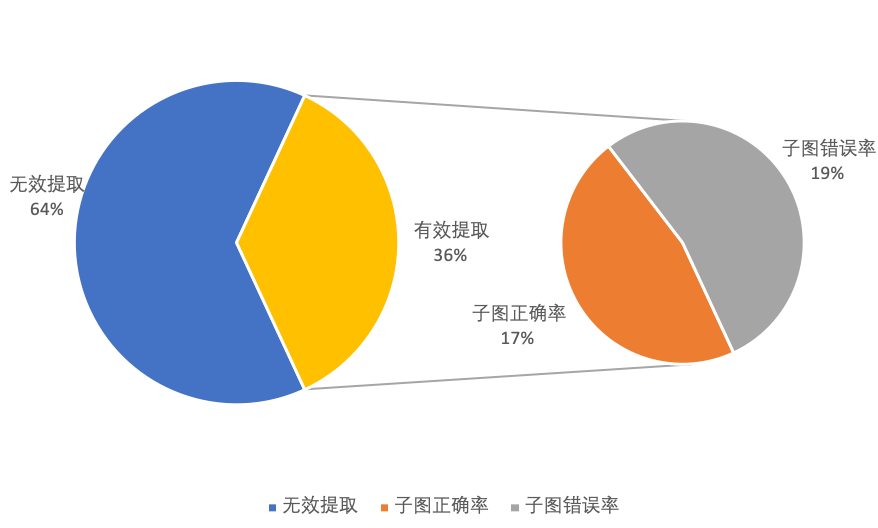
\includegraphics[width=0.8\textwidth]{kbsn_vqa.png}}
	\subfigure[KB-VQA]{
		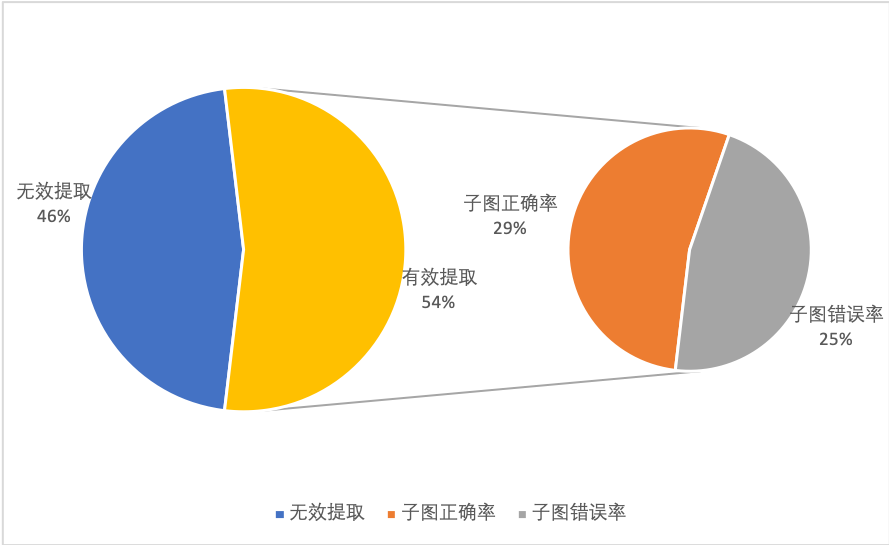
\includegraphics[width=0.8\textwidth]{kbsn_kb.png}}
	\caption{子图提取模块在两个数据集的表现}
	\label{kbsn_graph}
\end{figure}
\begin{table}[H]
% \resizebox{0.8\textwidth}{!}{}
\centering
\caption{知识子图提取模块在VQA2.0和KB-VQA数据集上的表现}
\begin{tabular}{ccc}
\toprule
指标 & VQA2.0 & KB-VQA \\
\midrule
子图参与率$jr$&  35.6& 54.3 \\
子图准确率$jc$&  46.5& 53.4 \\
\bottomrule
\end{tabular}
\label{kbsn_compr}
\end{table}

由图表可知,在KB-VQA数据集上,子图提取模块无论是参与率还是正确率都高于VQA2.0,这解释了KBSN与N-KBSN之间准确率之差在不同数据集上表现不同的原因。此外,子图提取模块在KB-VQA的子图参与率远高于在VQA2.0上的表现,这也说明KB-VQA的问题更加多样,且更复杂,因此能从中识别出更多的DBpedia实体。

\section{本章小结}
本章的主要内容是构建了一个基于知识库图嵌入的视觉问答模型(KBSN),并使用VQA2.0和KB-VQA两个差异明显的数据集训练和评估模型,实验结果证明了本文提出的知识库的图嵌入模块能提升模型的准确率。特别是在面对需要常识或者知识库的问题时,准确率提升更明显。

本章首先概括性地介绍了目前主流的知识库,随后详细介绍了本文提出的KBSN模型。其中,重点介绍了知识库子图提取和知识库子图嵌入的模型基础及架构。

为了获得好的知识库嵌入,本章进行了知识库嵌入实验。基于DBpedia知识库,本章通过一系列知识库预处理方法,构建了两个实验知识库:DBV和DBA,并使用了包括TransE在内的四个知识库嵌入模型在实验知识库上进行链路预测。实验结果证明了TransE模型能实现更好的知识库嵌入,并且本文构建的DBV知识库中的实体对应性很强,其知识库嵌入效果很好。

基于知识库嵌入的实验结果,本章使用KBSN模型在VQA2.0和KB-VQA数据集上进行视觉问答实验。实验结果显示,相较于N-KBSN,引入知识库嵌入的KBSN在两个数据集的准确率均有所提升,并且在KB-VQA上的提升非常明显。子图提取模块分析显示,相比于VQA2.0,子图提取模块在KB-VQA数据集上呈现出更高的子图参与率和子图正确率,这解释了KBSN在该数据集上的优异结果。






















